
Though trained on BNC data, the majority of data classified here is written directly for the web.  The impact this has upon classifier performance is not known, and insufficient gold standard data exists, tagged at sufficient resolution, to perform a direct evaluation.

Instead, data indexed by the Open Directory Project (DMOZ) was used as a measure of systematic bias.  The classification scheme used in DMOZ is significantly more diverse than that used in Lee's BNC index, covering a wider range of topics to a finer level of granularity.  As its goal is to represent a greater portion of the population than simply British English users this is unsurprising, however, it is organised hierarchically, and thus has larger-scale categories which are more compatible.

For each of the documents retrieved in the final corpus, an attempt was made to identify its DMOZ-equivalent category.  This was performed by matching URL or, failing such a detailed pattern, domain name, against 699,385 URLs taken from the publicly-accessible DMOZ archive.

For each BNC category (as assigned by the BNC45 model used in the retrieval task), the homogeniety of DMOZ categories was measured at each level of the hierarchy.  Categories below those which consist only of a single uppercase letter were concatenated, in order to remove some `A-Z' listing categories.


%Plots and tables.
The full set of 55,790 files downloaded for the BNC corpus comparison in Chapter~\ref{sec:evaluation} were used as source data.  Of these, 777 matched full-URL categories from the DMOZ classification, with a further 32,697 matching domain only.


% FIG HERE
\begin{figure}[h]
    \centering
    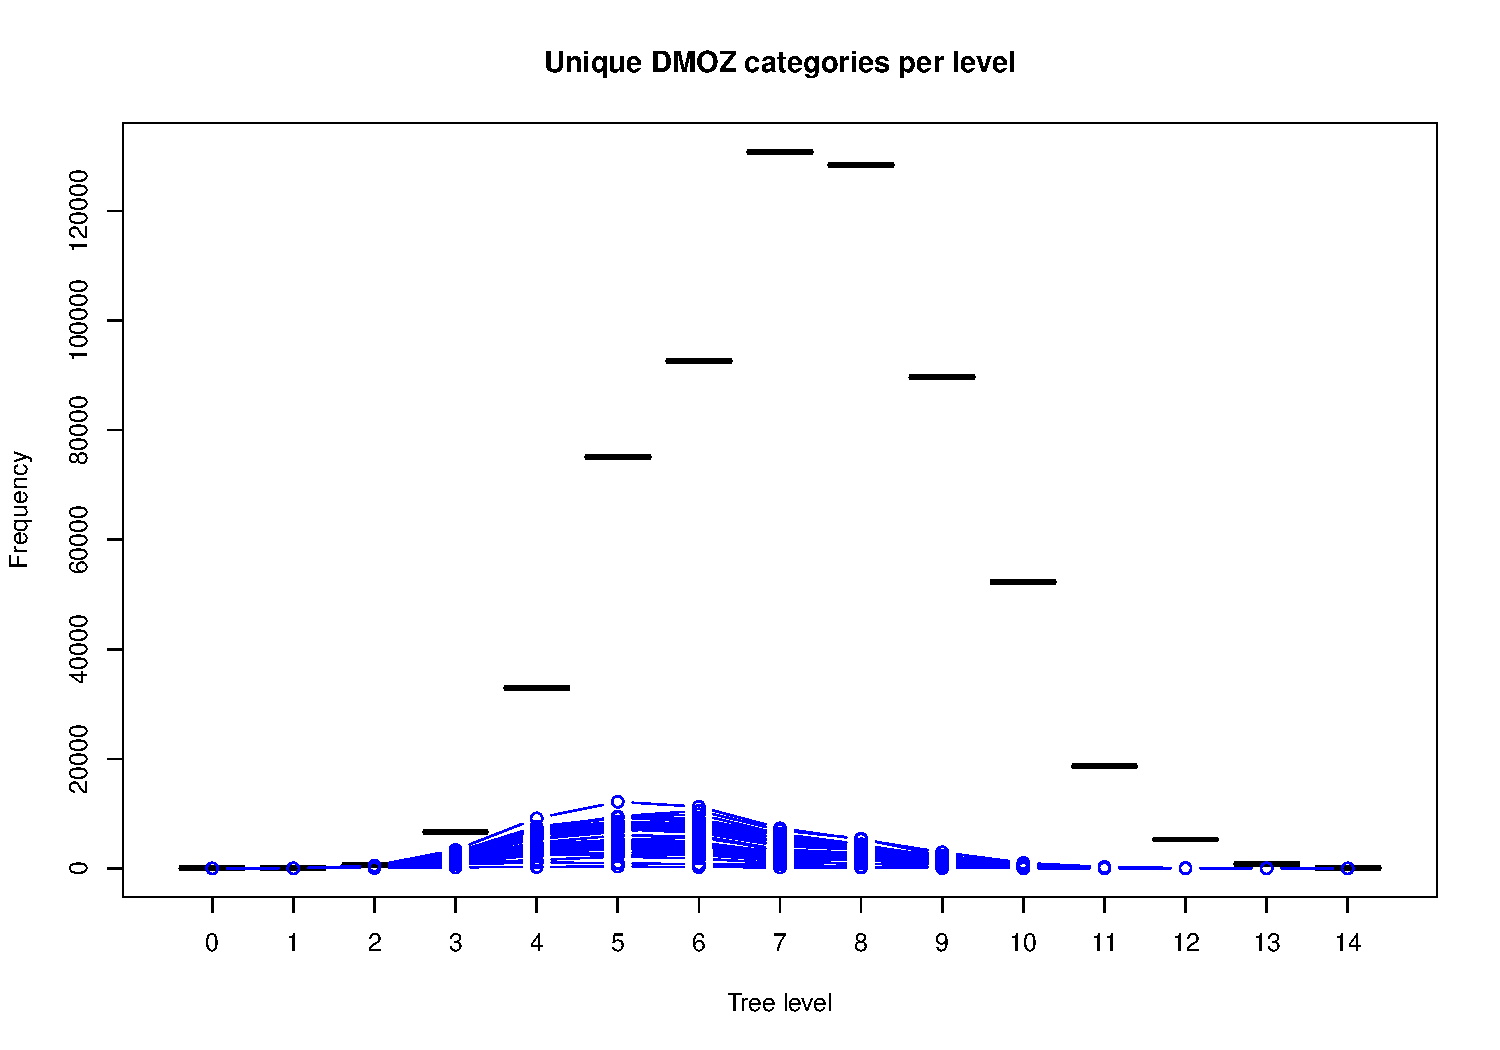
\includegraphics[width=0.9\textwidth]{appendices/dmozcounts}
    \caption{Unique category counts within and between BNC genres.}
    \label{fig:appendices:dmozcounts}
\end{figure}

The number of unique categories in the DMOZ overall is shown in Figure~\ref{fig:appendices:dmozcounts}.  The black lines illustrate the number of unique DMOZ categories at each level of the tree; the blue lines show the number of unique categories within each BNC genre, as classified by the BNC45 classifier model.


% FIG HERE
\begin{figure}[h]
    \centering
    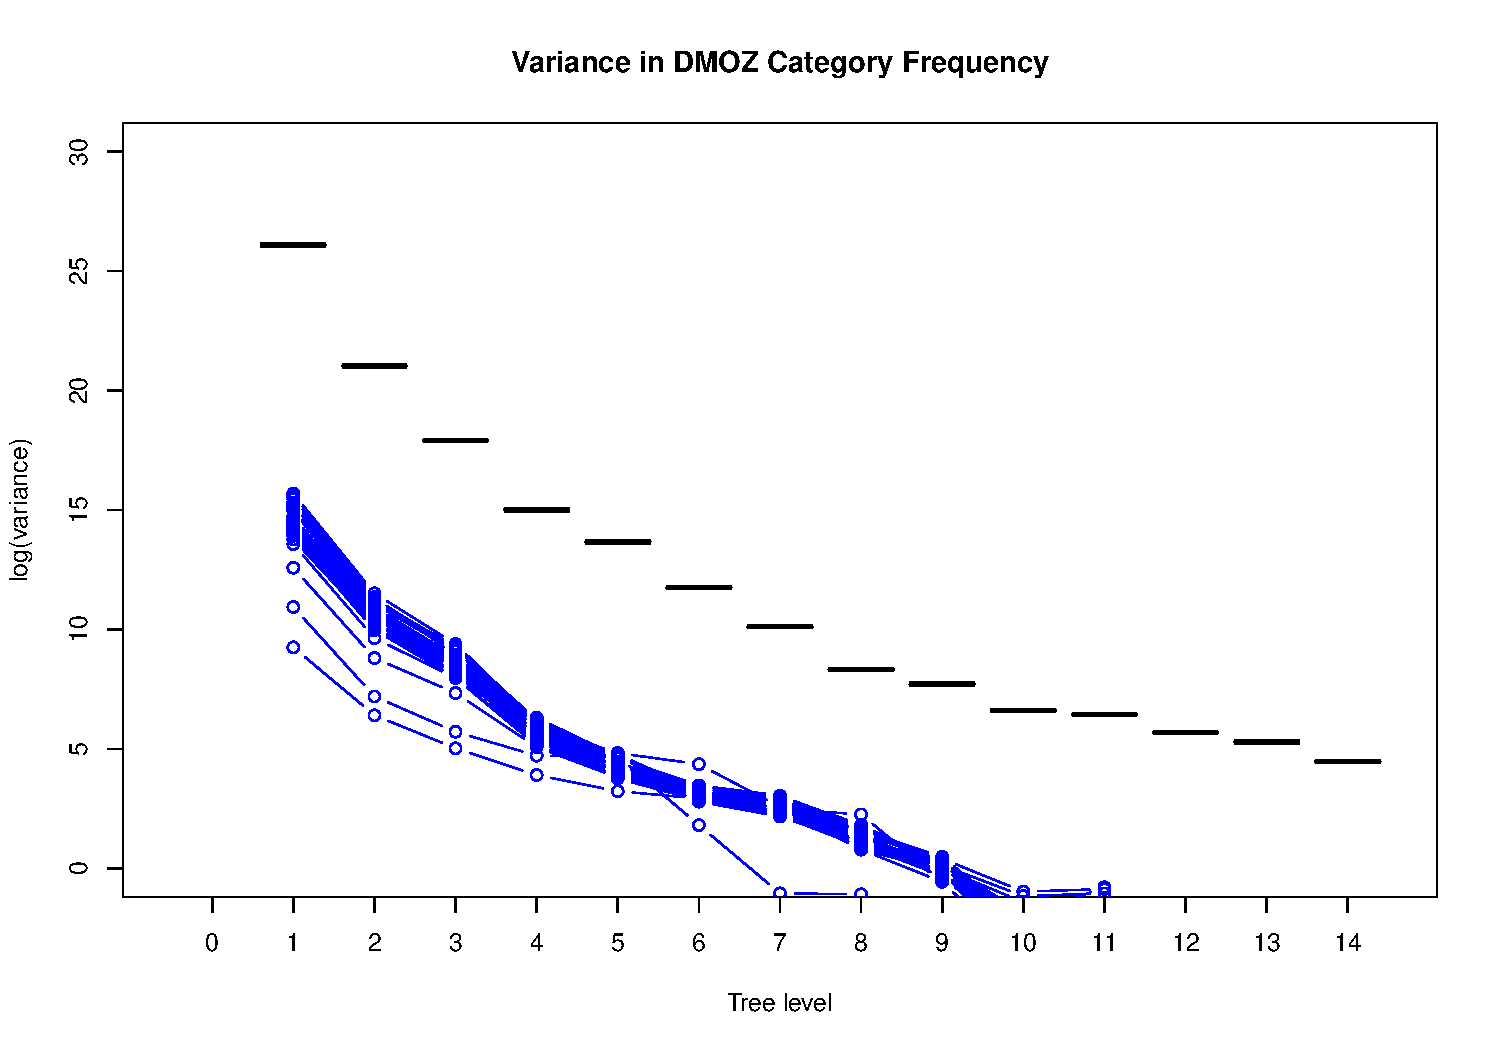
\includegraphics[width=0.9\textwidth]{appendices/dmozvars}
    \caption{Log variance in DMOZ category frequency across and within BNC genres}
    \label{fig:appendices:dmozvars}
\end{figure}

Figure~\ref{fig:appendices:dmozvars} shows log transformed variance in a similar manner.  Under ideal circumstances, where the BNC45 classifier is in perfect agreement with one level of the DMOZ across all categories, the variance remaining within each classifier will drop to zero at a given tree level.  Though this occurs for some values at a tree depth of around 10 for most genres, this is well beyond the bell curve of DMOZ classification, indicating that fewer DMOZ categories descend beyond this depth anyway.

% FIG HERE
\begin{figure}[h]
    \centering
    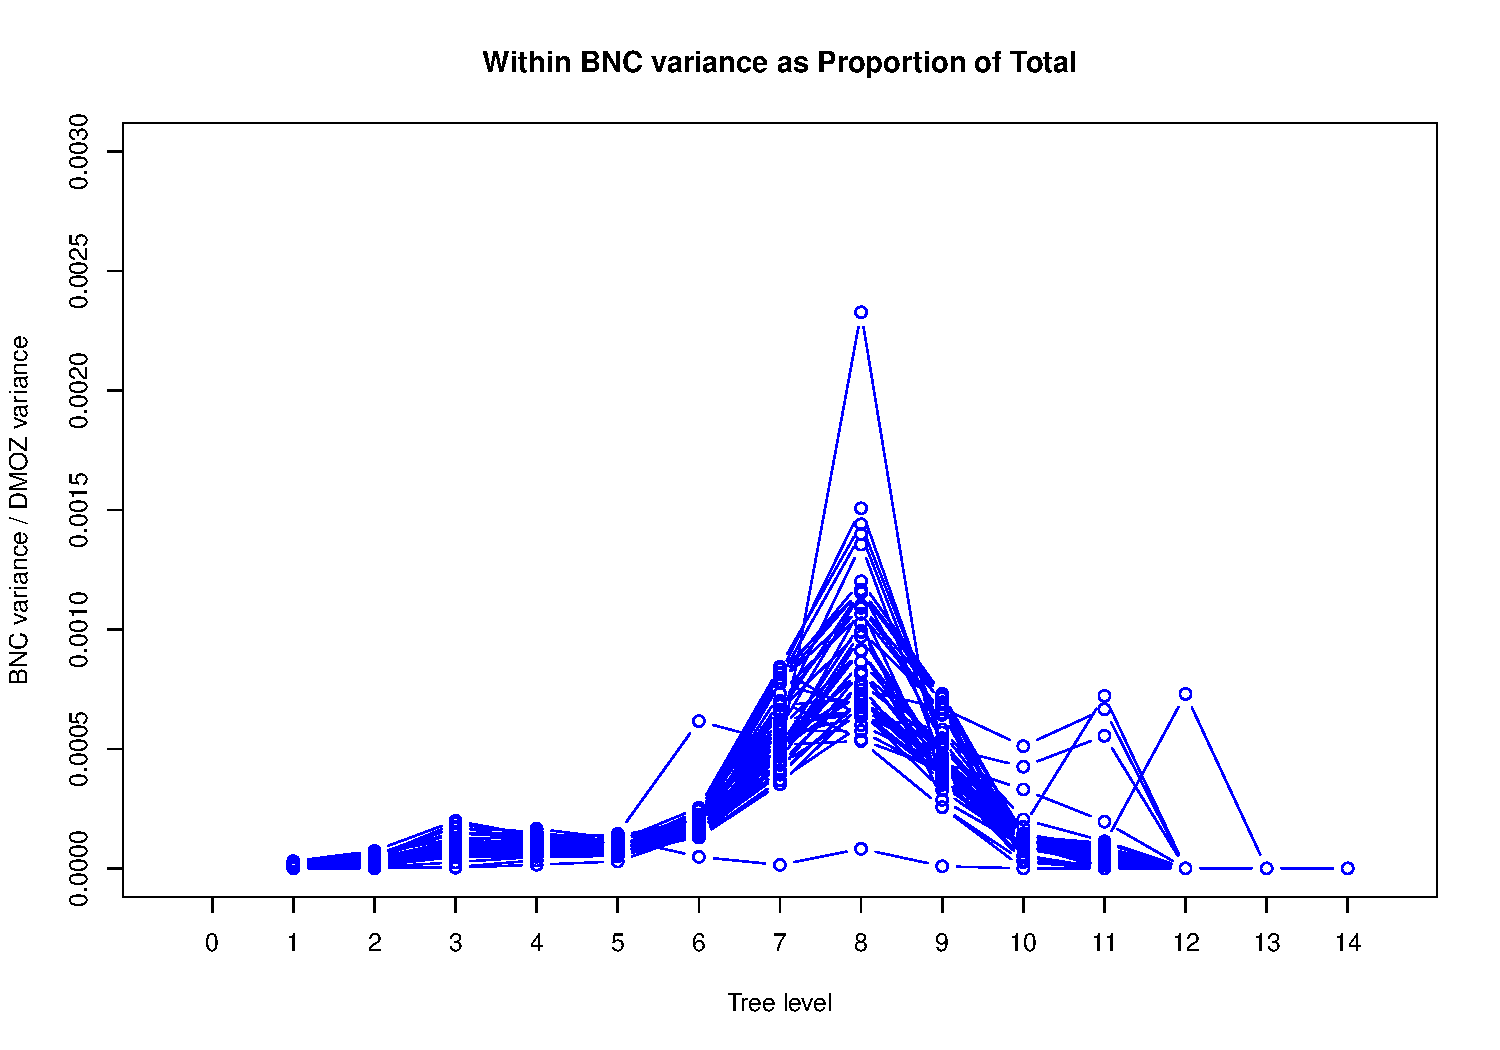
\includegraphics[width=0.9\textwidth]{appendices/dmozproportion}
    \caption{Within-genre DMOZ category frequency variance as a proportion of global variance}
    \label{fig:appendices:dmozproportion}
\end{figure}

\FloatBarrier

Figure~\ref{fig:appendices:dmozproportion} shows the proportion of variance within each BNC genre.  This displays a small reduction around a tree depth of five, mirroring the steepening of the curve in Figure~\ref{fig:appendices:dmozvars}.  This eclipsed by the relatively poor fit of later categories (as would be expected), before dropping off due to the smaller frequency of DMOZ categories beyond a tree depth of approximately ten.

These plots provide tentative evidence that best agreement between the DMOZ classification and the BNC45 classifier exists at a tree depth of around five.  It also indicates that the DMOZ classifications are potentially a useful tool in guiding retrieval of data, or, given sufficient human alignment, construction of gold standard data for further classifier evaluation.

%The main challenge would seem to be the variable tree depth for branches of the DMOZ tree, meaning that best agreement with other classification schemes is 

% The relative homogeniety of DMOZ classes for each BNC class may

